% =============================================================
%  MARBL Diagnostics Report
%  Verbatim LaTeX transcription of Diagnostics_report.docx
%  Packages: amsmath, booktabs, graphicx
% =============================================================

\documentclass[12pt, a4paper]{article}

% ── Packages ──────────────────────────────────────────────────
\usepackage{amsmath}
\usepackage{booktabs}

\usepackage{graphicx}
\graphicspath{{figures/}}

\usepackage{geometry}
\usepackage{microtype}
\usepackage{parskip}
\usepackage[hidelinks]{hyperref}

\hypersetup{
    bookmarksnumbered=true,    % Include section numbers in the navigation pane
    bookmarksopen=true,        % Expand the bookmark tree by default
    bookmarksopenlevel=1,      % How many levels to show open (1 = sections only)
    pdfstartview=FitH,         % Open the PDF fitting the width of the page
    pdfpagemode=UseOutlines,   % Force the navigation pane (outlines) to open on startup
    hidelinks                  % Removes those red boxes we discussed earlier
}

\geometry{
    top    = 2.5cm,
    bottom = 2.5cm,
    left   = 2.5cm,
    right  = 2.5cm
}

% ── Math shorthands ───────────────────────────────────────────
\newcommand{\WAPE}{\text{WAPE}}
\newcommand{\WAPECL}{\text{WAPE}_{\text{CL}}}



% ==============================================================
\begin{document}

\begin{titlepage}
    \centering

    \noindent
    \begin{minipage}[t]{0.5\textwidth}
        \raggedright
        
\includegraphics[width=5.5cm]{figures/wu_logo.png}
    \end{minipage}%
    \begin{minipage}[t]{0.5\textwidth}
        \raggedleft
        \raisebox{1cm}{
\includegraphics[width=5.5cm]{figures/marbl_logo.png}}
    \end{minipage}


    \vspace{1.8cm}

    {\LARGE\bfseries Regime Diagnostics \& Feature Enrichment for\\
    Day-Ahead Price Forecasts\par}

    \vspace{0.4em}

    {\large Intermediary Report\par}

    \vspace{2em}

    \begin{tabular}[t]{c@{\hspace{3em}}c}
        Pavle Cvijanovic  & Aleksandar Gradev \\[0.5em]
        Aleksandar Milosavljevic & Vincent Skakala
    \end{tabular}

    \vspace{2em}

    {\large \today\par}

\end{titlepage}

\tableofcontents
\newpage

% ==============================================================
\section{Introduction}
% ==============================================================
This report presents the intermediary results of the Marbl Energy Day-Ahead Price Forecast project. Building on the previous group’s forecasting pipeline, our work till now focused on improving both the data foundation and the diagnostic understanding of model performance across multiple European electricity markets.
We begin by extending and enriching the existing datasets, adding additional bidding zones and integrating variables. Alongside this, we replicate and revise the original modelling framework, identifying and resolving methodological issues such as data leakage to ensure a reliable evaluation baseline.
The core of the report is dedicated to a comprehensive set of model failure diagnostics. These analyses of last group’s model investigate where and why forecasting errors occur, examining performance across regimes, time structures, and market conditions. By decomposing errors and possibly identifying biases, we aim to uncover some limitations of the current modelling approach and provide a clear direction for our planned improvements.

% ==============================================================
\section{Summary of the previous project}
% ==============================================================

The previous group built an end-to-end price forecasting system covering three European
bidding zones: DK1 (Denmark West, wind-dominated), ES (Spain, solar-dominated), and
NO2 (Southern Norway, hydro-dominated).
The data pipeline follows a parallel ETL architecture with two independent processing
tracks- one for day-ahead prices from the ENTSO-E Transparency Platform and one for
ERA5 weather data from the Copernicus Climate Data Store- converging at a final merge
stage into a unified hourly masterset. Five variables form the feature set: temperature,
wind speed, solar irradiance, precipitation and the day-ahead price itself. The dataset
spans ten years (2015 - 2025), although the clustering and modelling are restricted to the
most recent three years to avoid mixing the low-volatility pre-2022 market regime with
the structurally different post-crisis period.
Pattern detection is performed using Ward linkage hierarchical clustering applied to
raw 24-dimensional daily price vectors. The number of clusters per zone was determined
jointly via elbow plots and acceleration diagnostics, yielding six clusters for DK1, three
for ES and five for NO2.
The forecasting architecture is a two-layer XGBoost system. Layer 1 is a multi-class
classifier that predicts the probability of each cluster occurring on a given day, using daily
weather aggregates, weekend and season dummy variables and three days of lagged mean
prices as inputs. Layer 2 consists of one regression model per cluster, predicting hourly
prices within that cluster using hourly weather variables and rolling precipitation windows
of 3, 7, 14, and 20 days, with 56 models in total. Final predictions are computed as a
probability-weighted average across all cluster-level forecasts.
Results were evaluated against two naive baselines using WAPE. The cluster model
3
achieved 31.45\% in DK1, outperforming both baselines. In ES and NO2 it came second,
behind the naive yesterday-repeat baseline, with WAPE scores of 33.84\% and 23.28\%
respectively. A Streamlit dashboard was also delivered, providing historical market
visualization, cluster analysis and day-ahead price forecasts driven by live weather API
data.




% ==============================================================
\section{Completed Data Integration}
% ==============================================================

For the data integration part, the goal was to create one enriched masterset per
country. The previous group had 3 mastersets (DK1, NO2, ES) which we extended
with new variables and also updated since their data only went up to November
2025. All mastersets have now been updated to include data up to March 2026. On
top of that, we built 2 completely new mastersets from scratch for DE-LU and FR,
bringing the total to 5 bidding zones as defined in our project proposal.

One challenge was the resolution mismatch. ENTSO-E and weather variables are
natively available at quarter-hourly resolution (4 entries per hour). We
standardized this by only taking the first entry of each hour.

The previous group only used day-ahead prices from ENTSO-E. We have tested and
prepared several additional ENTSO-E variables that are ready to be added to the
masterset: load forecasts, wind and solar generation forecasts, aggregated
electricity generation\ldots\ We are still deciding which ones to include and may
add more depending on what turns out to be useful for the model.

For the commodity prices we wanted to add TTF gas, CO\textsubscript{2} allowance
price and Brent crude as the fundamental price drivers described in Section 4.2.3
of the project plan. Finding a reliable free data source here was one of our main
challenges. All free official APIs we found had lag or weren't updated frequently
enough. We ended up using yfinance, a Python wrapper that scrapes live data from
Yahoo Finance. It updates daily when markets close, has no lag and is free. The
reliability risk is that if Yahoo Finance changes something on their end it might
break, however in practice this usually gets fixed within a day or two. These
yfinance variables are already added to the mastersets.

One specific issue was that the original EU ETS CO\textsubscript{2} ticker
(\textasciicircum ICEEUA) was delisted from Yahoo Finance, so we had to find an
alternative. We ended up with CO2.L, an ETC that physically holds EU allowances
and tracks the price closely, but it only goes back to October 2021. Since our
training window starts in 2022 this is sufficient, but if older data is needed we
would have to combine it with another source. We are planning to discuss potential
better data sources with Armin as mentioned in Section 4.2.4 of the project plan.

The second part of the data integration was building 2 new mastersets from
scratch for DE-LU and FR. This required downloading all ENTSO-E variables and
weather data in the same format as the previous group used. The weather data
download alone took 1134 minutes and 59 seconds for the period January 2023 to
March 2026.

% ==============================================================
\section{Summary of the Previous Group's Project}
% ==============================================================

We created a ``summary notebook'' which contains the entire code pipeline of the
previous group's project in one concise Jupyter notebook. For better readability,
most of the code was transferred to .py source files and wrapped in functions
which are called in the main notebook. This was done to effectively replicate
their results and to fix the data leakage issue and run the model failure
diagnostics.

% ==============================================================
\section{Data Leakage}
% ==============================================================

When we took over the previous group's forecasting pipeline, one of the first
things we identified was a data leakage occurring in two distinct places. These
leakages meant that the models had indirect access to information from the test
set during training, making their reported performance metrics unreliable and
overly optimistic.

The first source of leakage was in the clustering step. The previous group applied
Ward hierarchical clustering to the entire three-year dataset at once, including
the days that were later part of the test set. Because every day participates in
shaping the cluster centroids, the regime labels assigned to test days were
derived partly from the test data itself. In other words, the model ``knew''
future information when it assigned cluster labels, which then fed directly into
training the Layer 1 XGBoost classifier.

The second source of leakage was in the Layer 2 regression models. These 56
XGBoost models, each trained on a specific cluster, used cluster labels that had
themselves been contaminated by test-period observations. As a result, the
training data for Layer 2 was not truly isolated from future information either,
compounding the first bug.

Both occurrences were addressed systematically across all three bidding zones
(DK1, ES, NO2). For the clustering notebooks, we introduced a clean 70/30
train/test split before any clustering takes place. The Ward linkage algorithm
was then fitted exclusively on the training days. Test days were not clustered
directly, but their cluster assignments were determined by computing the nearest
training centroid and reconstructing the full label array from there. This ensures
that no test-day information ever influences the fitted clustering model. The same
fix was applied identically to all three pattern detection notebooks.

For the Predictions notebook we ensured the code pulls the clean leakage-free
outputs produced by the fixed clustering notebooks. We also introduced a
date-based cutoff for the Layer 2 training data, so those regression models are
trained strictly on pre-cutoff rows. An inner join on cluster labels was added to
drop any rows without a valid assignment.

Following our ``audit'', the $\WAPE$ numbers did not increase by much after the
fix, which was expected. Ward clustering computes centroids by averaging all
assigned days, and since the test set represents only around 15\% of the data
(approx.\ 160 days out of 1095 observations), each centroid was already dominated
by the 940 training days. The contamination from test days could shift any
centroid by at most 15\% and in practice most test days would have been assigned
to the same cluster anyway. This proved to us that Ward clustering leakage is
weaker than a typical supervised leakage, where a single mislabeled observation
can directly flip a decision boundary.

The conclusion is therefore that the leakage fix was methodologically correct,
but it was not the main driver of error in the original pipeline. The fix
nonetheless matters for two reasons - scientific integrity demands an honest
evaluation baseline and the Gaussian HMM approach we plan to implement next is
leakage-free by construction, so the clean pipeline is a necessary foundation.
The real performance gains are expected to come from feature enrichment (gas and
CO\textsubscript{2} prices, generation forecasts), autoregressive features in the
Layer 2 models and proper walk-forward cross-validation, all of which are the
next priorities on the roadmap.

% ==============================================================
\section{Model Failure Diagnostics}
% ==============================================================

% --------------------------------------------------------------
\subsection{Part 1: Breakdown by Cluster, Season, Weekday vs Weekend and by
price regime}
% --------------------------------------------------------------

\subsubsection{Aim}

This part of the model failure diagnostics establishes a performance baseline for
the XGBoost forecasting models across the three bidding zones (DK1, ES, NO2).
These diagnostics decompose model performance along four structural dimensions -
cluster, season, day type, and price regime - to identify where errors
concentrate.

The analysis exposes a known failure mode of standard $\WAPE$ when applied to
electricity prices, and replaces it with a corrected metric throughout.

\subsubsection{The metric fix - Clamped WAPE}

Standard $\WAPE$ divides total absolute error by the sum of absolute actual
prices. In electricity markets, actual prices frequently approach or fall below
zero, causing the denominator to collapse and $\WAPE$ to inflate arbitrarily -
not because the model is bad, but because the metric breaks down. The diagnostics
replace standard $\WAPE$ with clamped $\WAPE$ ($\WAPECL$), which enforces a
minimum absolute price floor of $\delta = 10$ EUR/MWh in the denominator while
leaving the numerator unchanged. Any slice where raw $\WAPE$ and $\WAPECL$
diverge substantially is flagged as a metric artefact rather than a genuine model
failure.

\subsubsection{Diagnostics description and findings}

For each zone, the pipeline computes MAE, raw $\WAPE$, clamped $\WAPE$, and
signed bias (mean of predicted minus actual) across four breakdowns (see \emph{Figure 1}, \emph{Figure 2}, \emph{Figure 3}):

\textbf{Cluster breakdown: } Performance is evaluated separately for each regime cluster
assigned by the hierarchical clustering model. This distinguishes whether high
aggregate error is driven by a specific regime type - for instance, a cluster
characterised by extreme prices or atypical weather - or is spread evenly across
all regimes.


\textbf{Result: }The worst-performing cluster differs by zone: Cluster 2 in DK1,
Cluster 1 in ES, and Cluster 2 in NO2 each record the highest clamped $\WAPE$
within their respective zones. The concentration of error within specific clusters
rather than being evenly distributed suggests the failures are regime-specific,
pointing toward either Layer 1 misclassification routing days into the wrong
regime, or Layer 2 regression weakness within those regimes.

% \begin{figure}[ht]
% \centering
% \includegraphics[width=0.8\textwidth]{placeholder}
% \caption{Clamped WAPE per cluster for DK1, ES, and NO2}
% \end{figure}

\textbf{Seasonal breakdown: }Errors are grouped by season to test whether model weaknesses
are concentrated in particular times of year. Given that the test set covers only
the second half of the year, this breakdown is included for completeness but is
noted as structurally limited.

\textbf{Result: }No meaningful seasonal pattern emerges across any of the three
zones. Summer and autumn $\WAPE$ figures are closely aligned in DK1, ES, and
NO2, indicating that the model's weaknesses are structural rather than tied to a
particular time of year. This breakdown is also limited by the test set covering
only the second half of the year.

% \begin{figure}[ht]
% \centering
% \includegraphics[width=0.8\textwidth]{placeholder}
% \caption{Seasonal WAPE breakdown for DK1, ES, and NO2}
% \end{figure}

\textbf{Weekday vs. weekend breakdown: } Performance is computed separately for weekdays
and weekends. A consistent weekday/weekend gap across zones would indicate a
structural missing feature, i.e., possibly weekend demand suppression.

\textbf{Result: }All three zones show consistently higher clamped $\WAPE$ on
weekends compared to weekdays. The uniformity of this pattern across zones with
fundamentally different generation mixes suggests a shared missing feature. A
weekend dummy variable alone is insufficient to model this.

% \begin{figure}[ht]
% \centering
% \includegraphics[width=0.8\textwidth]{placeholder}
% \caption{Weekday vs.\ weekend clamped WAPE for DK1, ES, and NO2}
% \end{figure}

\textbf{Price bucket breakdown: } Hours are grouped into four regimes: negative prices,
near-zero prices (0-20 EUR/MWh), normal prices, and spike prices (top 5\% by
zone). This is a diagnostically informative breakdown, as it directly tests
whether the model fails specifically in the tail regimes that matter most for
trading.

\textbf{Result: }This is the most informative result. Negative and near-zero
price hours produce by far the largest errors in every zone, while normal-regime
hours are forecast considerably more accurately. The pattern is consistent across
DK1, ES, and NO2, pointing to a shared root cause: the model lacks supply-side
features: wind generation in DK1, solar in ES, hydro reservoir levels in NO2,
that would allow it to anticipate the renewable oversupply conditions under which
low and negative prices occur.

% --- DK1 Plot ---
\begin{figure}[H] % [H] forces it to stay EXACTLY here
    \centering
    
\includegraphics[width=0.95\textwidth]{diagnostic_DK1}
    \caption{Breakdown for DK1}
\end{figure}

% --- ES Plot ---
\begin{figure}[H]
    \centering
    
\includegraphics[width=0.95\textwidth]{diagnostic_ES}
    \caption{Breakdown for ES}
\end{figure}

% --- NO2 Plot ---
\begin{figure}[ht]
    \centering
    
\includegraphics[width=0.95\textwidth]{diagnostic_NO2}
    \caption{Breakdown for NO2}
\end{figure}



\subsubsection{Cross-zone comparison}

A final summary table consolidates the four key metrics at the aggregate level
across all three zones, providing a single-row-per-zone comparison that situates
the breakdown results in context. The inflation check additionally identifies
every slice where raw $\WAPE$ exceeded clamped $\WAPE$ by more than 20 percentage
points, distinguishing genuine forecasting failures from metric breakdowns.

\textbf{Result: }NO2 is the best-performing zone overall (MAE 15.87,
$\WAPECL$ 23.52\%), DK1 sits in the middle ($\WAPECL$ 30.94\%), and ES is the
hardest to forecast ($\WAPECL$ 33.41\%). The signed bias column is particularly
informative: DK1 is nearly unbiased at $+0.31$ EUR/MWh, ES carries a substantial
positive bias of $+10.03$ EUR/MWh reflecting systematic over-prediction, and NO2
shows a moderate negative bias of $-3.63$ EUR/MWh.

\begin{table}[ht]
    \centering
    \small
    \caption{Cross-zone aggregate performance summary (test set).
             Signed bias is mean (predicted $-$ actual) in EUR/MWh.}
    \label{tab:cross_zone}
    \begin{tabular}{@{}lcccc@{}}
        \toprule
        \textbf{Zone}
            & \textbf{MAE}
            & $\boldsymbol{\WAPE}$\textbf{(\%)}
            & $\boldsymbol{\WAPECL}$\textbf{(\%)}
            & \textbf{Signed Bias (EUR/MWh)} \\
        \midrule
        DK1 & 24.75   & 31.35 & 30.94 & $+0.31$  \\
        ES  & 23.12   & 34.03 & 33.41 & $+10.03$ \\
        NO2 & 15.87 & 23.66 & 23.52 & $-3.63$  \\
        \bottomrule
    \end{tabular}
\end{table}

\textbf{Metric validation. }A quick inflation check confirms that the failures on negative and
near-zero price hours are genuine rather than artefacts of the denominator
problem. Even after clamping, $\WAPECL$ remains between 251\% and 416\% for
negative price hours and between 316\% and 378\% for near-zero hours across all
three zones. The raw figures are far worse: ES reaches 7,693\% raw $\WAPE$ on
negative price hours, collapsing to 416\% once clamped, a 7,277 percentage point
inflation. This confirms that raw $\WAPE$ must not be reported for these buckets,
and that clamped $\WAPE$ is the only reliable metric in low-price regimes.

% \begin{figure}[p]
% \centering
% 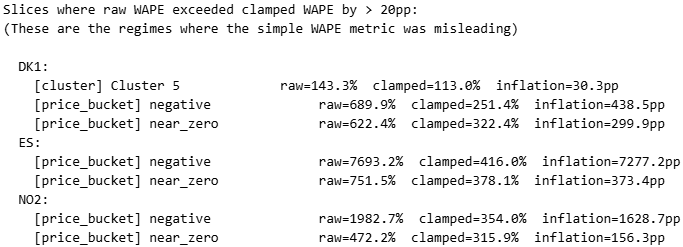
\includegraphics[width=0.8\textwidth]{inflation_check}
% \caption{Raw WAPE vs.\ clamped WAPE inflation check by price bucket and zone}
% \end{figure}

% --------------------------------------------------------------
\subsection{Part 2: Signed Bias Analysis by Hour of Day and Price Regime}
% --------------------------------------------------------------

\subsubsection{Aim}

Where the Point 1 diagnostics measure how large errors are across market regimes,
the Part 3 diagnostics examine their direction and timing. The central question is
whether the model's errors are random or they are systematic functions of the hour
of day and the price regime.

\subsubsection{Diagnostics description and findings}

The analysis constructs a unified residual frame - predicted minus actual for
every test hour across all three zones, and subjects it to three complementary
decompositions.

\textbf{Plot A - Signed hourly bias.} (see \emph{Figure 4}).
For each zone, the mean residual is computed
for every hour of the day (0-23) and plotted as a continuous line against the
zero-bias reference. This reveals whether the model systematically over- or
under-predicts at particular times, and whether the bias reverses sign within a
single day. The peak and trough hours are annotated directly on the chart to
anchor the zone-specific narratives. The plot uses mean residual as the primary
statistic as it represents the expected EUR cost of bias per traded MWh integrated
across all market conditions.

\textbf{Result: }The bias profiles across all three zones are non-random and
follow patterns consistent with the physical generation mix of each market. In
DK1, the model is broadly unbiased in the early morning but turns sharply negative
from midday onward, peaking at $-43.0$ EUR/MWh at hour 17. In ES, the model
over-predicts heavily during morning hours, peaking at $+35.3$ EUR/MWh at hour
09, then reverses into under-prediction during the evening ramp between 18:00 and
21:00 - a sign reversal within a single day that is consistent with insufficient
signal for both the midday solar supply surplus and the subsequent sunset ramp. In
NO2, under-prediction is spread broadly across the afternoon and evening, peaking
at $-18.8$ EUR/MWh at hour 17, without the sharp intraday peak observed in DK1
and ES. This pattern is consistent with a missing slow-moving driver such as hydro
reservoir levels or cross-border flow variables.

\begin{figure}[ht]
\centering

\includegraphics[width=1\textwidth,height=0.8\textheight, keepaspectratio]{p3_hourly_bias}
\caption{Plot A: Mean signed hourly residual (EUR/MWh) for each hour of the
         day (0--23) for DK1, ES, and NO2, with peak and bottom annotated}
\end{figure}

\textbf{Plot B - Intraday bias faceted by price bucket.}(see \emph{Figure 5}) The same hourly residual
profiles are recomputed separately within each of four price regimes: negative
prices, near-zero prices (0-20 EUR/MWh), normal prices, and spike prices (top 5\%
of actual prices per zone). This separates the structural intraday pattern from
the regime-specific one, and in particular isolates whether spike under-prediction
is uniformly distributed across the day or concentrated in specific hours. Missing
data points in certain hour-bucket combinations reflect the absence of observations
in that regime at that hour, not imputation.

\textbf{Result: }The price regime decomposition reveals two structurally opposite
failure modes that are consistent across all three zones. In the negative and
near-zero price buckets, all residuals are substantially positive - ranging between
20 and 80 EUR/MWh. In the spike bucket, residuals are almost entirely negative,
reaching below $-100$ EUR/MWh, confirming systematic under-prediction of price
peaks. The normal price bucket is the only regime where residuals hover near zero,
though a visible drift into under-prediction persists during evening hours across
all zones. ES shows the highest intraday volatility in residuals, with a
particularly pronounced over-prediction spike around 06:00 - 09:00 in the
low-price buckets.

\begin{figure}[ht]
\centering

\includegraphics[width=\textwidth]{p3_small_multiples}
\caption{Plot B: Intraday mean residual profiles faceted by price regime
         (negative, near-zero, normal, spike) for DK1, ES, and NO2}
\end{figure}

\textbf{Plot C - Spike hit-rate.}(see \emph{Figure 6}) For each zone, all test hours
falling above the zone-specific spike threshold (the 95th percentile of actual
prices) are isolated. Three under-prediction thresholds are then applied -
residual below $-10$, $-20$, and $-50$ EUR/MWh - and the share of spike hours
breaching each threshold is reported. This shows out of every spike event the
model was asked to forecast, what fraction it missed. The result is a direct
measure of model conservatism under the market conditions where accurate
forecasting has the highest financial stakes.

\textbf{Result: }The spike hit-rate analysis confirms that under-prediction during
extreme price events is pervasive and severe. Across all three zones, the model
under-predicts at least 85\% of spike hours by more than 10 EUR/MWh. DK1 shows
the worst performance at the tail: 65.7\% of its spike hours are missed by more
than 50 EUR/MWh, with a mean residual of $-77$ EUR/MWh on hours already above the
144.7 EUR/MWh spike threshold. ES is considerably better at the extreme end: only
18.7\% of Spanish spike hours are missed by more than 50 EUR/MWh. NO2 sits
between the two at 28.1\%.

\begin{figure}[ht]
\centering

\includegraphics[width=0.8\textwidth]{p3_spike_hit_rate}
\caption{Table C / Plot C: Spike under-prediction hit-rates at thresholds of
         $-10$, $-20$, and $-50$ EUR/MWh for DK1, ES, and NO2}
\end{figure}

\textbf{Plot D - Weekday vs. weekend split.}(see \emph{Figure 7}) The hourly mean residual profiles
from Plot A are recomputed separately for weekdays and weekends, displayed as
solid and dashed lines respectively, with the MAE for each day type reported in
the title. This tests whether the model's intraday bias pattern is stable across
day types, or whether weekend demand dynamics, which differ structurally from
weekday patterns due to reduced industrial load, produce a distinct and worse error
profile.

\textbf{Result: }The weekday/weekend split produces the sharpest finding in ES,
where MAE deteriorates from 21.5 EUR/MWh on weekdays to 31.5 EUR/MWh on weekends
- a 46\% increase. The weekend curve is uniformly elevated across all morning
hours, peaking around 08:00 - 09:00 at approximately $+55$ EUR/MWh.DK1 shows
almost no weekday/weekend difference (MAE 24.7 vs. 25.3). NO2 shows a moderate
gap (14.4 vs. 19.1), with the weekend curve exhibiting a sharper and earlier
midday peak, though the mechanism is less clear-cut than in ES.

\begin{figure}[ht]
\centering

\includegraphics[width=0.8\textwidth]{p3_weekend_weekday}
\caption{Plot D: Mean signed hourly residual split by weekday (solid) and
         weekend (dashed) for DK1, ES, and NO2, with MAE per day type in title}
\end{figure}

% --------------------------------------------------------------
\subsection{Part 3: Intraday Volatility Diagnostic}
% --------------------------------------------------------------

With this diagnostic we aim to examine the intraday dynamics in the researched
markets and understand in more details where do the models fail.

We start by looking if the models can reproduce the intraday volatility structure
of actual electricity prices. Intraday volatility is computed for each day as the
variation in hourly prices within that day, capturing how turbulent or stable the
market was. First, we will look at the timeseries of the daily intraday volatility
of both actual and predicted prices over the full evaluation (testing) period. We
want to check whether the model systematically underestimates or overestimates
turbulence and whether it can capture high-volatility events. Second, we will
compare the mean intraday volatility of the actual price against the mean
volatility produced by each individual predicted cluster, exposing whether the
cluster architecture itself introduces a structural smoothing bias.

After that we will investigate the relationship between market turbulence and
forecast error quality. For each day in the test set, actual intraday volatility
is plotted against the forecast MAE for that day in a scatterplot. Both axes share
the same unit (EUR/MWh), making the relationship directly interpretable. The
purpose is to test whether the model's forecast errors are systematically driven
by high-volatility days or whether errors are distributed uniformly regardless of
market conditions. A positive relationship would confirm that the model's
performance degrades specifically under turbulent market conditions, linking the
structural findings of Diagnostic 2 directly to measurable forecasting
consequences.

\subsubsection{Findings}

\paragraph{Intraday Volatility Time Series} (see \emph{Figure 8, Figure 9, Figure 10})

Across all three bidding zones, the plots reveal a consistent and systematic
pattern: The weighted predicted price substantially underestimates actual intraday
volatility throughout the entire evaluation period. The two lines rarely converge
and the gap is not random. The predicted volatility is persistently and
structurally lower than actual volatility in every zone.

The smoothing bias is universal but its severity differs by zone. DK1 and ES show
predicted volatility that to an extent tracks the general movement of the actual
series, even if it misses the spikes. NO2 is the most extreme case - the predicted
volatility is nearly flat at near-zero throughout the whole period, while actual
volatility oscillates substantially and ends with a dramatic spike above 80
EUR/MWh.

Across all zones, high-volatility spike days are completely invisible to the
model. These are not marginal misses - the predicted series simply does not react
to turbulent market events, suggesting the cluster architecture cannot represent
the conditions that produce such days. This is consistent across all three zones
and across the entire evaluation window, confirming this is not a seasonal or
zone-specific occurence but a fundamental limitation of the model design.

\begin{figure}[p]
\centering
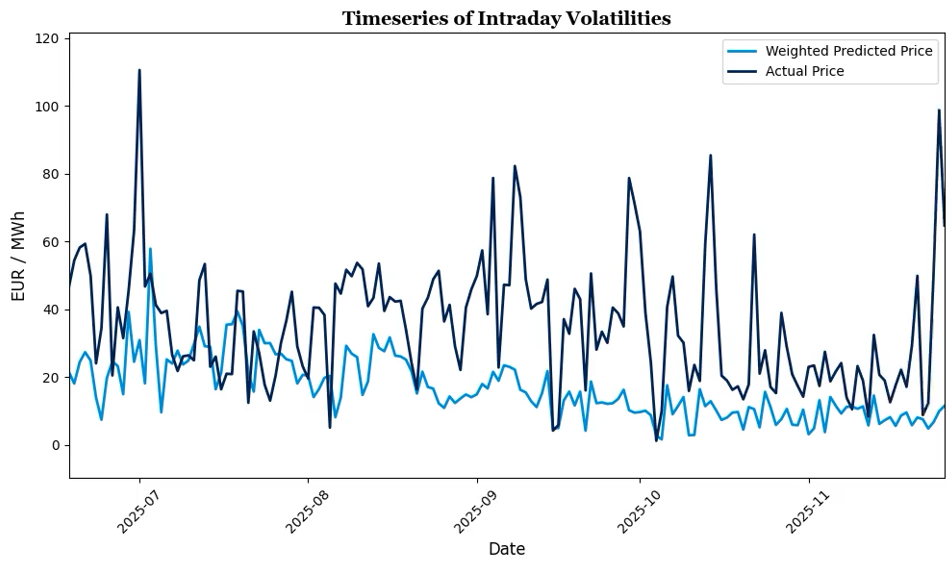
\includegraphics[width=\textwidth]{intraday_vol_DK1}
\caption{Intraday volatility time series: actual vs.\ predicted for DK1 over the full evaluation period}
\end{figure}

\begin{figure}[p]
\centering
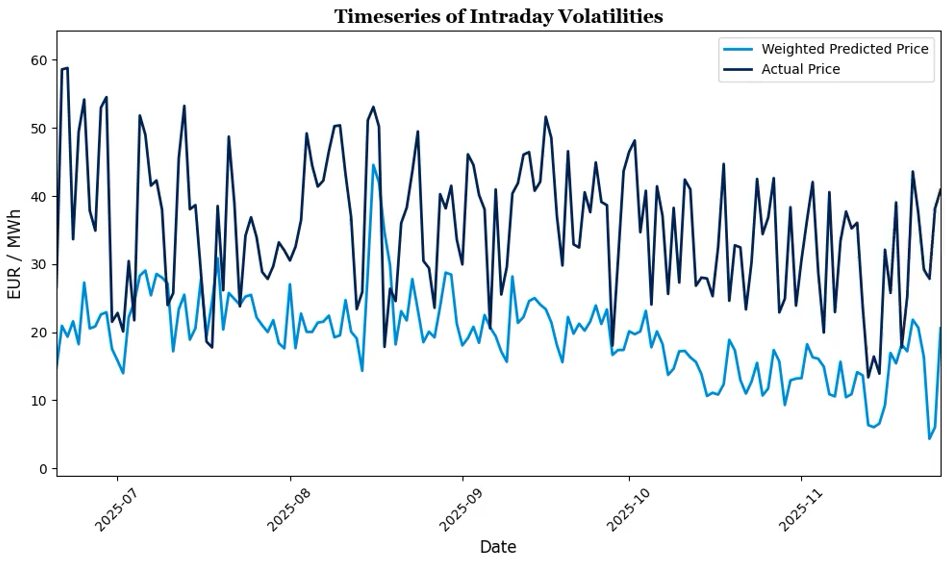
\includegraphics[width=\textwidth]{intraday_vol_ES}
\caption{Intraday volatility time series: actual vs.\ predicted for ES over the full evaluation period}
\end{figure}

\begin{figure}[h]
\centering
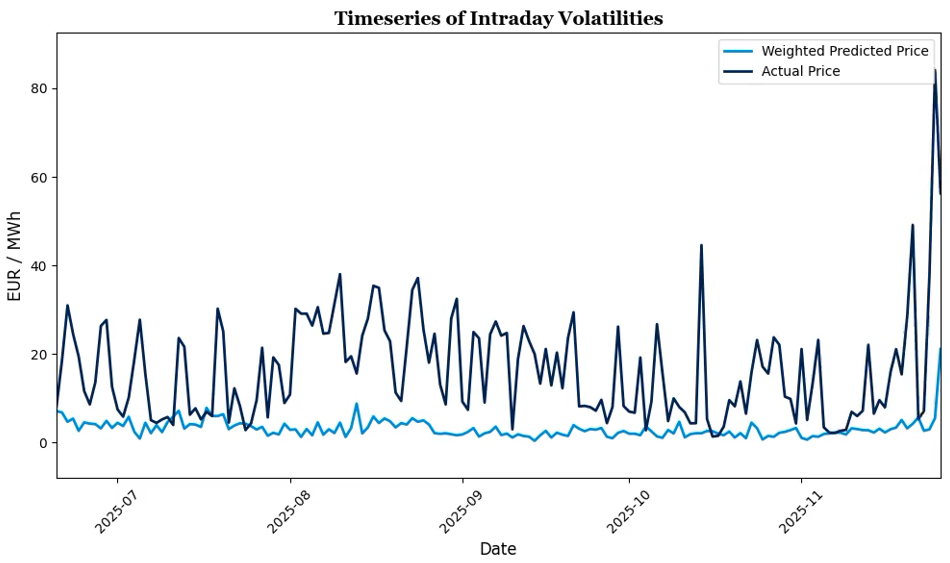
\includegraphics[width=\textwidth]{intraday_vol_NO2}
\caption{Intraday volatility time series: actual vs.\ predicted for NO2 over the full evaluation period}
\end{figure}


\paragraph{Intraday Volatility vs MAE} (see \emph{Figure 11, Figure 12, Figure 13})

Across all three bidding zones, a positive relationship between actual intraday
volatility and forecast error is visible, confirming that high-volatility days are
systematically harder for the current models to forecast. This is consistent with
the timeseries diagnostic, which showed the model is structurally unable to
reproduce intraday price spikes. The scatterplots now quantify the consequence:
turbulent days do not just produce wrong volatility estimates, they produce
substantially higher absolute forecast errors.

However, the strength of this relationship varies considerably across zones. In
DK1 and NO2 the positive trend is relatively clear and concentrated, whereas in
ES the point cloud is much more dispersed with high MAE values appearing even at
low volatility levels. This divergence is important as it indicates that intraday
volatility is not the sole driver of forecast error across all markets. In DK1 and
NO2 model fails specifically when the market is turbulent, while in ES it fails
more broadly and independently of market conditions. This also points to deeper
structural issues in the forecasting model.

A notable observation across all three plots is the presence of notable outliers
at extreme volatility levels, where both actual volatility and MAE are far above
the typical range. These outliers represent the most challenging market days and
confirm that the current models have no mechanism to adapt to exceptional market
conditions.

\begin{figure}[p]
\centering
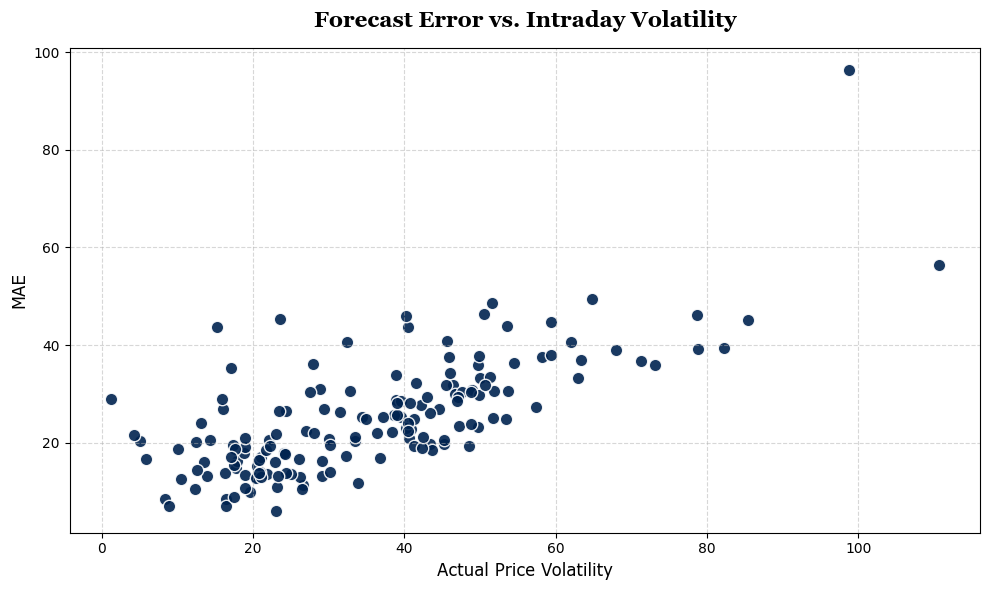
\includegraphics[width=\textwidth]{mae_vs_volatility_DK1}
\caption{Actual volatility vs MAE for DK1}
\end{figure}

\begin{figure}[p]
\centering
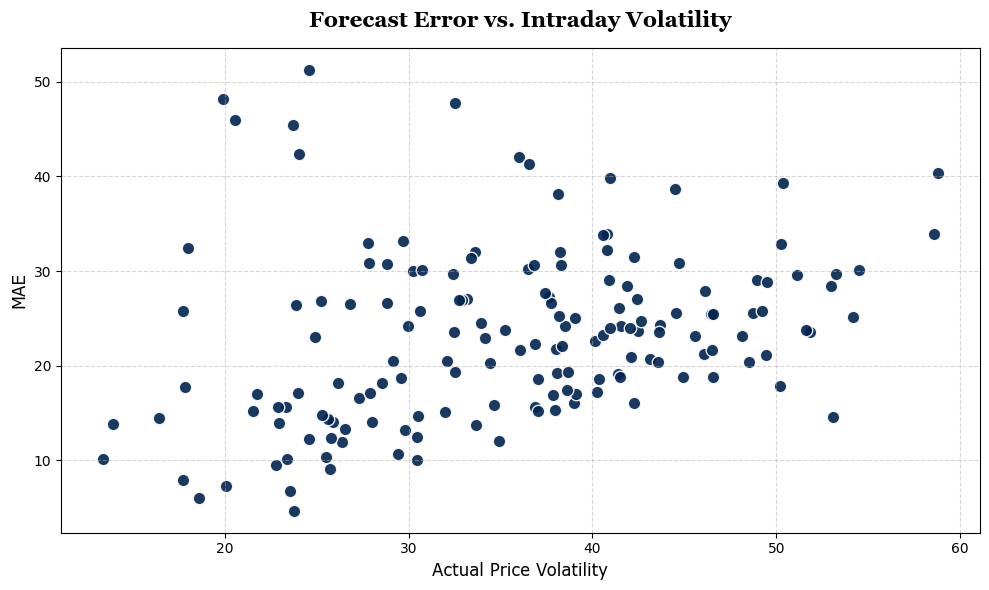
\includegraphics[width=\textwidth]{mae_vs_volatility_ES}
\caption{Actual volatility vs MAE for ES}
\end{figure}

\begin{figure}[h]
\centering
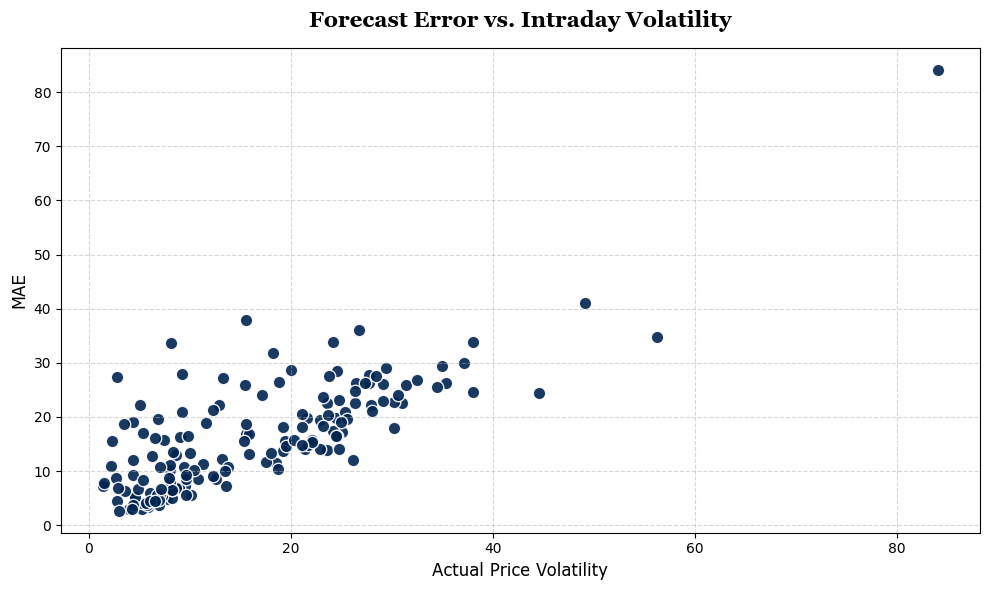
\includegraphics[width=\textwidth]{mae_vs_volatility_NO2}
\caption{Actual volatility vs MAE for NO2}
\end{figure}


\paragraph{Mean Intraday Volatility for Actual Price vs. Predicted Clusters} (see \emph{Figure 14, Figure 15, Figure 16})

The dominant pattern across DK1 and ES is consistent with the timeseries
findings: every individual cluster systematically underestimates the actual mean
intraday volatility. In both zones the actual volatility sits at approximately 35
EUR/MWh, while all predicted clusters fall well this level regardless of which
cluster is assigned. This confirms that the smoothing bias observed in the
timeseries is not driven by one poorly defined cluster but is a structural property
shared across all clusters.

NO2 tells a strikingly different and revealing story. Four of the five clusters
produce near-zero mean volatility, dramatically below the actual level of c.a.\
16.5 EUR/MWh. However, Cluster 5 alone produces a mean volatility of
$\sim$36.5 EUR/MWh, which highly exceeds the actual mean.

\begin{figure}[p]
\centering
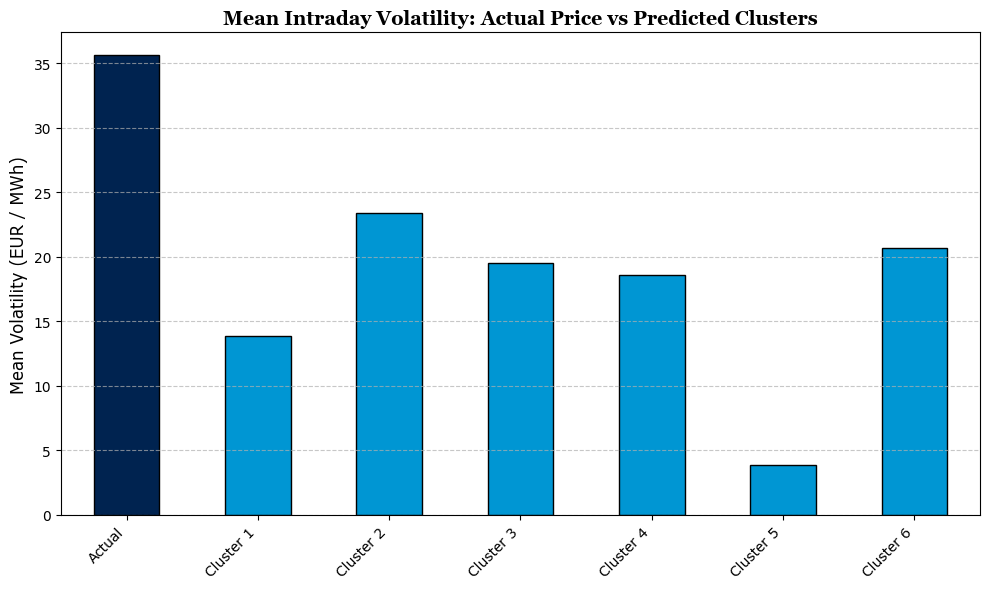
\includegraphics[width=\textwidth]{mean_intraday_volatility_DK1}
\caption{Comparison of Mean intraday volatility between actual price and predicted clusters for DK1}
\end{figure}

\begin{figure}[p]
\centering
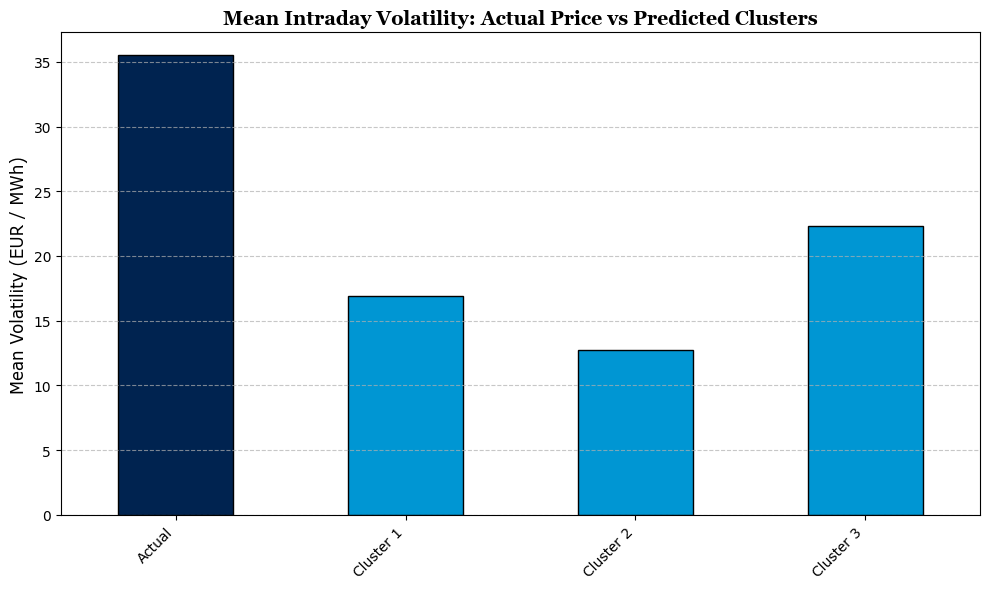
\includegraphics[width=\textwidth]{mean_intraday_volatility_ES}
\caption{Comparison of Mean intraday volatility between actual price and predicted clusters for ES}
\end{figure}

\begin{figure}[h]
\centering
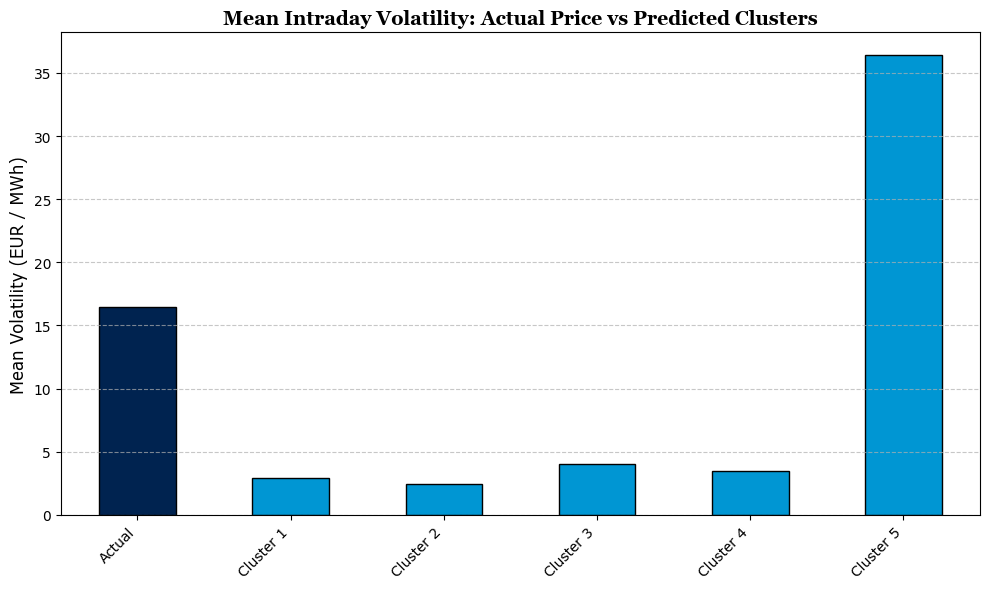
\includegraphics[width=\textwidth]{mean_intraday_volatility_NO2}
\caption{Comparison of Mean intraday volatility between actual price and predicted clusters for NO2}
\end{figure}


% --------------------------------------------------------------
\subsection{Part 4: Layer 1 vs Layer 2 Error Diagnostic}
% --------------------------------------------------------------

The current MARBL forecasting model consists of Layer 1 (regime classifier that
gives cluster probabilities) and Layer 2 (separate forecaster that generates
hourly price forecasts per cluster).

This diagnostic isolates which component is causing forecast errors. We split test
results into two groups: days where Layer 1 correctly predicted the cluster
(assigned the highest probability to the correct cluster) versus days where it was
wrong. By comparing forecast accuracy ($\WAPE$, Mean Absolute Error) between
these groups, we identify whether Layer 1's regime misclassification or Layer 2's
forecasting within clusters is the primary bottleneck.

\subsubsection{Findings}

% \begin{table}[H]
%     \centering
%     \caption{Layer 1 vs.\ Layer 2 Error Diagnostic: accuracy and $\WAPE$ by zone.}
%     \label{tab:layer_diagnostic}
%     \begin{tabular}{@{}lcccc@{}}
%         \toprule
%         \textbf{Zone}
%             & \textbf{Top-1 Accuracy (\%)}
%             & \textbf{Top-3 Accuracy (\%)}
%             & $\boldsymbol{\WAPE}$ \textbf{Correct (\%)}
%             & $\boldsymbol{\WAPE}$ \textbf{Incorrect (\%)} \\
%         \midrule
%         DK1 & 59.26 & 96.30  & 30.76 & 33.40 \\
%         ES  & 81.25 & 100.00 & 33.76 & 36.07 \\
%         NO2 & 56.88 & 99.38  & 19.08 & 31.71 \\
%         \bottomrule
%     \end{tabular}
% \end{table}

\paragraph{Top-1 vs Top-3 Accuracy}

The gap between Top-1 and Top-3 accuracy is the first key finding. In all three
zones, the correct cluster falls within the classifier's top 3 predictions almost
perfectly. However, top-1 accuracy is considerably lower. This means the
classifier consistently identifies the right neighbourhood of regimes but struggles
to commit to the correct one.

We believe this is a direct consequence of the overlapping cluster centroids. Ward
linkage produces clusters that are not well-separated, so the decision boundary
between adjacent regimes is genuinely ambiguous. Our proposed Gaussian HMM
addresses this by design, as its probabilistic regime assignments naturally handle
boundary uncertainty.

% \begin{figure}[ht]
% \centering
% \includegraphics[width=0.6\textwidth]{placeholder}
% \caption{Top-1 vs.\ Top-3 Layer 1 classification accuracy for DK1, ES, and NO2}
% \end{figure}

\paragraph{WAPE Gap Between Correct and Incorrect Cluster Days}

The $\WAPE$ difference between days where Layer 1 was correct and days where it
was incorrect varies substantially across zones, and this variation is the most
actionable finding of this diagnostic.

In NO2, the gap is 12.6 percentage points (19.1\% vs 31.7\%). This is by far the
largest gap across all three zones, meaning that Layer 1 misclassification is
disproportionately costly here. When the classifier assigns the wrong regime, the
Layer 2 regression model produces predictions that are structurally misaligned with
the actual price profile. Fixing Layer 1 through the HMM transition is therefore
the highest-priority intervention for NO2.

In DK1 and ES, the gap is narrow, 2.6pp and 2.3pp respectively. Even when Layer 1
assigns the wrong cluster, the $\WAPE$ barely changes. This tells us that in these
two zones, the clusters are similar enough in their price profiles that a wrong
assignment does not dramatically worsen the regression output. The error is not
coming from regime misclassification, but from within the Layer 2 regression
models themselves, regardless of which cluster is assigned. The bottleneck in DK1
and ES is therefore Layer 2 feature poverty, i.e.\ the absence of gas prices, load
forecasts and zone-specific supply variables that the regression models need to
produce accurate hourly predictions within any regime.

% \begin{figure}[ht]
% \centering
% \includegraphics[width=0.8\textwidth]{placeholder}
% \caption{Clamped WAPE split by Layer 1 correct vs.\ incorrect classification
%          for DK1, ES, and NO2}
% \end{figure}

\end{document}
